
\subsubsection{Задача прогнозирования}
Эвристическое утверждение, на котором основывается решение задачи
$pred$ в ООМ, является более общим случаем утверждения
(\ref{assertORS1}):
\begin{assert}
	\label{assertORS2}
	Если два объекта схожи, то заданные им оценки близости пользователя будут
	приблизительно равны. \cite{rs-handbook,melville}.
\end{assert}
Данное утверждение является более общим случаем утверждения ООМ
(\ref{assertORS1}),
которое
используется при решении задачи $topN$,
так как рассматривает любые оценки, поставленные пользователем,
а не только те, которые означают, что между пользователем и объектом
выполняется отношение близости.

Во введенной терминологии данное утверждение примет следующий вид:
\begin{equation}
	i \rt j \Leftrightarrow |\rho(u,i) - \rho(u,j)|
	\le \varepsilon_p
\end{equation}

Правило вывода ООМ для решения задачи $pred$ запишется следующей
формулой:
\begin{equation}
	\label{ors-pi-p}
	\rh(u_a, i_{\bot}) = g_p(\{\rho(u_a, i^{\prime}_0)\}),
	i^{\prime}_0 \rt i_{\bot}.
\end{equation}
Правило вывода говорит о том, что оценки близости между
пользователем $u_a$ и объектами, являющимися соседями,
функционально связаны. Таким образом, зная
оценки близости, которые пользователь уже задал объектам
$i \rt i_{\bot}$, можно вычислить $\rh(u_a, i_{\bot})$
на основании функциональной связи
$g_p$.

Схема решения задачи $pred$ заключается в построении кластера
$\nip = \{ i_0 : i_0 \rt i_{\bot}\}$, центром которого является прогнозируемый
объект $i_{\bot}$. Решение задачи $pred$ запишется в виде:
\begin{equation}\label{pred-f}
	\rh(u_a,i_{\bot}) = g_p(\{\rho(u_a, i_0): i_0 \in \nip \}
\end{equation}
где $g_p$ --- некоторая функция, используемая в модели для
формирования по множеству оценок пользователя прогнозной оценки.

%===================================================================
%--------------------------------------------
%===================================================================
Опишем возможную\footnote{Модели могут отличаться такими параметрами, как,
например, функция $\di$, поэтому нижеописанная модель является одной из
возможных}
реализацию ООМ
\footnote{
	На данном этапе без оценки качества $\mathcal{E}_{topN}$
	}
 и на ее примере решим
задачу прогнозирования  \cite{item-based} %TODO: set cite. I think need
												%to see amazon
\begin{itemize}
	\item $c_X(u_a) = \{\rho(u_a,i_0)\}$
	\item $c_Y = (y_1,...,y_{|Y|})$;
	\item $\di(i,j) = \cos(\angle(c_Y(i),c_Y(j)))$
\end{itemize}
\bigbreak

Прогнозирование строится на основании оценок, поставленных активным пользователем
объектам, между которыми и прогнозируемым выполняется отношение близости.
Поиск таких объектов может осуществляться линейно по значениям, которые уже
хранятся в матрице мер близости $\mathbb{M}$, находящихся в строке с порядковым
номером, соответствующим индексу объекту. После построения кластера соседей
$\nip$,
вычисляется значение {\it прогнозной функции} от оценок пользователей,
поставленных $i \in \nip$.


На рисунке (\ref{dia:p-ors}) изображена блок-схема алгоритма
решения задачи $pred$ в ООМ.
\begin{figure}[htb]
	\caption{Блок-схема алгоритма построения матрицы $\mathcal{M}$}
\begin{center}
	\label{dia:p-ors}
 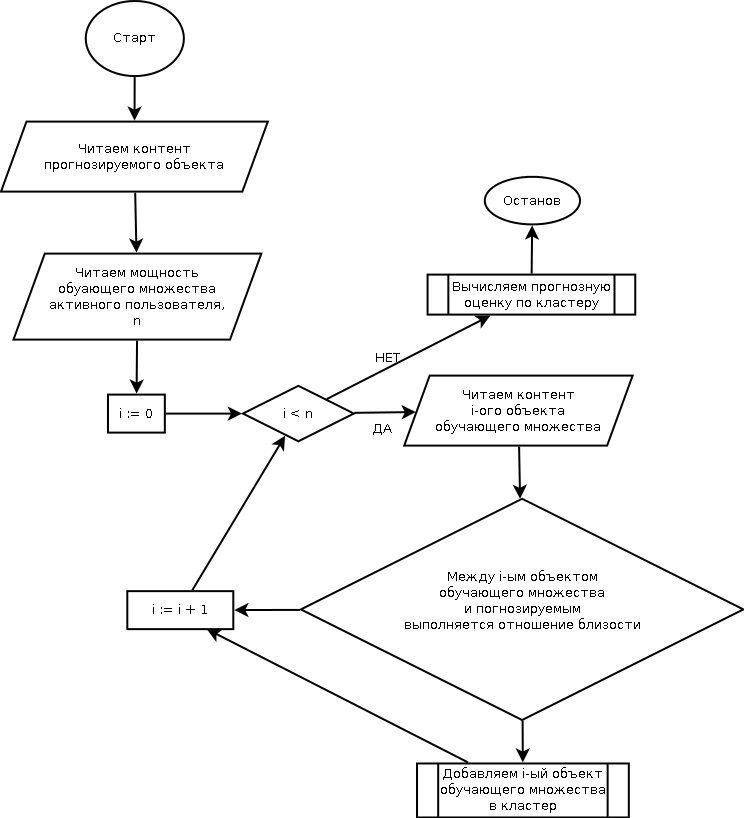
\includegraphics[width=7in,height=8in]{pics/algs/p-ors.png}
\end{center}
\end{figure}
Блок-схеме алгоритма решения задачи $pred$ в ООМ соответствует
псевдокод, представленный на изображении <<Стандартный алгоритм решения задачи $pred$ в ООМ>>  (\ref{alg:p-ors}).

\begin{figure}[htb]
\caption{Стандартный алгоритм решения задачи $pred$ в ООМ}
\label{alg:p-ors}
	%\begin{algorithm}
\begin{algorithmic}[1]
\State $\nip \gets \varnothing$\Comment{Множество объектов,
	оцененных активным пользователем и схожих с прогнозируемым объектом}
	\State $l \gets i_{\bot}$\Comment{Сохраняем в переменной $l$ индекс
	прогнозируемого объекта}
	\State $P^a \gets \varnothing$ \Comment{Множество оценок близости
	активного пользователя}
	\For {$i \in I^a_0$}
	\If {$\mathbb{M}^i_l \ge \Delta_i$}\Comment{Объект $i$ близок к
	прогнозируемому}
  \State $\nip \gets \nip \bigcup \{ i \}$
	\State $P^a \gets P^a \bigcup \{\rho(u_a,i)\}$
  \EndIf
\EndFor
\State $\rh(u_a,i) \gets g_p( P^a )$\Comment{Рассчитываем значение функции прогнозирования}
\end{algorithmic}
%\end{algorithm}
\end{figure}
